\documentclass[aspectratio=169,12pt]{beamer}
\usepackage[utf8]{inputenc}
\usepackage{graphicx}
\usepackage{tikz}
\usepackage{pgf-pie}
\usepackage{listings}
\usepackage{hyperref}
\usepackage{booktabs}
\usepackage{multicol}
\usepackage{xcolor}
\usepackage{fontawesome5}
\usepackage{verbatim}

\usetheme{Madrid}
\usecolortheme{whale}
\setbeamertemplate{navigation symbols}{}

\definecolor{codegreen}{rgb}{0,0.6,0}
\definecolor{codegray}{rgb}{0.5,0.5,0.5}
\definecolor{codepurple}{rgb}{0.58,0,0.82}
\definecolor{backcolour}{rgb}{0.95,0.95,0.92}
\definecolor{alertred}{rgb}{0.8,0.1,0.1}
\definecolor{alertgreen}{rgb}{0.1,0.8,0.1}
\definecolor{owaspyellow}{RGB}{255,140,0}

\lstdefinestyle{mystyle}{
    backgroundcolor=\color{backcolour},   
    commentstyle=\color{codegreen},
    keywordstyle=\color{magenta},
    numberstyle=\tiny\color{codegray},
    stringstyle=\color{codepurple},
    basicstyle=\ttfamily\footnotesize,
    breakatwhitespace=false,         
    breaklines=true,                 
    captionpos=b,                    
    keepspaces=true,                 
    numbers=left,                    
    numbersep=5pt,                  
    showspaces=false,                
    showstringspaces=false,
    showtabs=false,                  
    tabsize=2
}
\lstset{style=mystyle}

% Define languages used in listings (fallback-safe)
\lstdefinelanguage{Go}{
  morekeywords={package,import,func,return,if,else,for,range,type,struct,map,var,const,interface,select,case,break,continue,goto,default,defer,go,chan},
  sensitive=true,
  morecomment=[l]{//},
  morecomment=[s]{/*}{*/},
  morestring=[b]",
}
\lstdefinelanguage{JavaScript}{
  morekeywords={import,export,from,async,await,return,if,else,for,while,const,let,var,function,class,extends,constructor,super,try,catch,finally,new,delete,typeof,instanceof,in,of,yield,case,break,continue,default,throw},
  sensitive=true,
  morecomment=[l]{//},
  morecomment=[s]{/*}{*/},
  morestring=[b]",
  morestring=[b]',
  morestring=[b]`,
}

\title{Day 2: OWASP Top 10 Threats and Mitigation Strategies}
\subtitle{Comprehensive Training with Practical Examples and Hands-on Exercises}
\author{Security Training Team}
\institute{Web Application Security Department}
\date{\today}

\begin{document}

\begin{frame}
\titlepage
\end{frame}

% ===== New: Hands-on Focused Section =====
\begin{frame}{Agenda Hari 2 (Praktik + Teori)}
\begin{itemize}
\item Tujuan: Memahami risiko OWASP Top 10 melalui praktik langsung
\item Teori ringkas tiap risiko: akar masalah, skenario serangan, dampak
\item Lab terarah: langkah eksploitasi aman dan mitigasi terukur
\item Review hasil lab: indikator keberhasilan dan cara verifikasi
\item Mini-CTF dan rubric penilaian
\end{itemize}
\end{frame}

\begin{frame}{Prasyarat \& Setup Lingkungan}
\begin{columns}
\column{0.5\textwidth}
\textbf{Perangkat yang dibutuhkan}
\begin{itemize}
\item Docker Desktop (Windows/Mac/Linux)
\item PowerShell atau Terminal Bash
\item OWASP ZAP / Burp (opsional)
\item Postman atau curl
\end{itemize}
\textbf{Garis besar arsitektur}
\begin{itemize}
\item Aplikasi target: DVWA, Juice Shop, WebGoat
\item Tools DAST: OWASP ZAP baseline scan
\item Proxy debugging: Burp/ZAP
\end{itemize}
\column{0.5\textwidth}
\textbf{Variabel lingkungan (contoh)}
\begin{itemize}
\item \texttt{DB\_PASSWORD}, \texttt{REDIS\_PASSWORD}
\item \texttt{SESSION\_SECRET}
\item \texttt{MONGODB\_URI} / \texttt{DATABASE\_URL}
\end{itemize}
\textbf{Catatan keamanan}
\begin{itemize}
\item Jalankan hanya di lingkungan lab terisolasi
\item Jangan menggunakan data produksi
\end{itemize}
\end{columns}
\end{frame}

\begin{frame}[fragile]{Docker Compose: Lab Mandiri}
\textbf{Jalankan seluruh target dan tools secara lokal}
\begin{lstlisting}
version: '3.8'
services:
  dvwa:
    image: vulnerables/web-dvwa
    ports:
      - "8080:80"

  juiceshop:
    image: bkimminich/juice-shop
    ports:
      - "3000:3000"

  webgoat:
    image: webgoat/webgoat-8.2
    ports:
      - "8081:8080"

  zap:
    image: owasp/zap2docker-stable
    command: zap-baseline.py -t http://dvwa:80 -I
    depends_on:
      - dvwa
\end{lstlisting}
\textbf{Perintah}
\begin{itemize}
\item \texttt{docker compose up -d}
\item Akses: DVWA (\texttt{http://localhost:8080}), Juice Shop (\texttt{http://localhost:3000}), WebGoat (\texttt{http://localhost:8081/WebGoat})
\end{itemize}
\end{frame}

\begin{frame}{Metodologi Pengujian}
\begin{columns}
\column{0.5\textwidth}
\textbf{Pendekatan}
\begin{itemize}
\item SAST: analisis kode statis
\item DAST: uji black-box aplikasi berjalan
\item IAST: sensor di dalam aplikasi saat runtime
\item Threat modeling: STRIDE, data flow
\end{itemize}
\column{0.5\textwidth}
\textbf{Definisi Keberhasilan}
\begin{itemize}
\item Dapat mereproduksi kerentanan secara aman
\item Menerapkan mitigasi dan memverifikasi perbaikan
\item Menulis catatan uji dan rekomendasi
\end{itemize}
\end{columns}
\end{frame}

% ===== A01: Broken Access Control =====
\begin{frame}{A01: Broken Access Control - Teori}
\begin{itemize}
\item Akar masalah: pemeriksaan otorisasi tidak konsisten atau hilang
\item Pola umum: IDOR, bypass otorisasi, force browsing, mass assignment
\item Dampak: kebocoran data, modifikasi data pengguna lain
\item Strategi: verifikasi otorisasi server-side di tiap aksi dan objek
\end{itemize}
\end{frame}

\begin{frame}[fragile]{A01: Lab - IDOR dan Cek Otorisasi}
\textbf{Target:} DVWA (modul File atau View Profile)
\begin{enumerate}
\item Login sebagai user biasa, catat \textit{request} untuk melihat profil: \texttt{/vulnerabilities/view\_user.php?id=2}
\item Ubah parameter \texttt{id} menjadi milik user lain (mis. \texttt{1}) via Burp Repeater
\item Observasi apakah data user lain terlihat (indikator IDOR)
\item \textbf{Mitigasi:} tambahkan middleware cek kepemilikan sumber daya
\end{enumerate}
\vspace{0.2cm}
\textbf{Contoh middleware (Express.js)}
\begin{lstlisting}[language=JavaScript]
// Pastikan resource dimiliki oleh user yang login
function authorizeOwnership(getOwnerIdFromResource) {
  return async (req, res, next) => {
    try {
      const resourceId = req.params.id;
      const ownerId = await getOwnerIdFromResource(resourceId);
      if (!req.user || String(req.user.id) !== String(ownerId)) {
        return res.status(403).json({ error: 'Forbidden' });
      }
      next();
    } catch (e) { next(e); }
  };
}
// Penggunaan: router.get('/users/:id', authorizeOwnership(getOwner), handler)
\end{lstlisting}
\end{frame}

\begin{frame}[fragile]{A01: Snippet Go + JS (ESM)}
\begin{columns}
\column{0.5\textwidth}
\textbf{Go: Middleware kepemilikan (net/http)}
\begin{lstlisting}[language=Go]
type OwnerFunc func(id string) (string, error)

func AuthorizeOwnership(getOwner OwnerFunc, next http.Handler) http.Handler {
  return http.HandlerFunc(func(w http.ResponseWriter, r *http.Request) {
    userID := r.Header.Get("X-User-ID") // contoh: hasil auth sebelumnya
    id := r.URL.Query().Get("id")
    ownerID, err := getOwner(id)
    if err != nil || userID == "" || ownerID != userID {
      http.Error(w, "forbidden", http.StatusForbidden)
      return
    }
    next.ServeHTTP(w, r)
  })
}
\end{lstlisting}
\column{0.5\textwidth}
\textbf{JS (ESM): Hindari kepercayaan sisi-klien}
\begin{lstlisting}[language=JavaScript]
// modules/validate.js
export function isValidId(v){ return /^\d+$/.test(v); }

// app.js (ESM)
import { isValidId } from './modules/validate.js';
const id = new URLSearchParams(location.search).get('id');
if (!isValidId(id)) alert('Invalid');
// CATATAN: Otorisasi wajib di server, ESM ini hanya usability.
\end{lstlisting}
\end{columns}
\end{frame}

% ===== A04: Insecure Design (Lab) =====
\begin{frame}{A04: Lab - Threat Modeling \& Secure Design}
\textbf{Tujuan:} Mengidentifikasi abuse case dan kontrol desain yang hilang.
\begin{enumerate}
\item Pilih satu fitur (mis. upload file atau reset password)
\item Gambar data flow sederhana: sumber data, proses, penyimpanan, trust boundary
\item Identifikasi ancaman (STRIDE): spoofing, tampering, repudiation, info disclosure, DoS, elevation of privilege
\item Tentukan kontrol: validasi, autentikasi, otorisasi, rate limit, logging, enkripsi
\item Verifikasi kontrol pada implementasi (code/config review singkat)
\end{enumerate}
\textbf{Artefak:} DFD ringkas + daftar kontrol yang dipilih + rencana uji.
\end{frame}

\begin{frame}[fragile]{A02: Snippet Go - TLS \& HSTS}
\textbf{Go server dengan TLS modern + HSTS}
\begin{lstlisting}[language=Go]
srv := &http.Server{ Addr: ":443" }
http.HandleFunc("/", func(w http.ResponseWriter, r *http.Request){
  w.Header().Set("Strict-Transport-Security", "max-age=31536000; includeSubDomains")
  w.Header().Set("X-Content-Type-Options", "nosniff")
  w.Header().Set("X-Frame-Options", "DENY")
  w.Header().Set("Content-Security-Policy", "default-src 'self'")
  fmt.Fprintln(w, "ok")
})
// Pastikan sertifikat disediakan; gunakan reverse proxy jika perlu
log.Fatal(srv.ListenAndServeTLS("server.crt", "server.key"))
\end{lstlisting}
\end{frame}

% ===== A06: Vulnerable and Outdated Components (Lab) =====
\begin{frame}[fragile]{A06: Lab - Dependency \& SBOM Scanning}
\textbf{Langkah:}
\begin{enumerate}
\item Pindai dependencies proyek contoh (Node/Python/Java)
\item Hasilkan SBOM dan scan untuk CVE
\item Terapkan update minor/patch, verifikasi kompatibilitas
\end{enumerate}
\textbf{Perintah contoh}
\begin{lstlisting}
# Node.js
npm ci
npm audit --audit-level=high || true
osv-scanner --lock package-lock.json || true

# Python
pip install -r requirements.txt
pip-audit || true

# Java (Maven)
mvn -DskipTests org.owasp:dependency-check-maven:check || true

# SBOM + scan container/artifact
syft dir:. -o cyclonedx-json > sbom.json
grype sbom:sbom.json || true
\end{lstlisting}
\textbf{Go (tambahan)}
\begin{lstlisting}
go mod tidy
go list -m -u all            # cek update module
govulncheck ./... || true    # scan CVE modul Go
go mod verify                # verifikasi checksum
\end{lstlisting}
\textbf{Kriteria Sukses:} daftar CVE prioritas + PR update + bukti build lulus.
\end{frame}

% ===== A08: Software and Data Integrity Failures (Lab) =====
\begin{frame}[fragile]{A08: Lab - Supply Chain Integrity}
\textbf{Langkah:}
\begin{enumerate}
\item Verifikasi integritas artefak container dengan Sigstore Cosign
\item Validasi signature webhook (HMAC) di aplikasi
\item Kunci dependency ke lockfile dan aktifkan verifikasi di CI
\end{enumerate}
\textbf{Cosign verify (contoh)}
\begin{lstlisting}
COSIGN_EXPERIMENTAL=1 cosign verify ghcr.io/org/app:latest \
  --certificate-oidc-issuer https://token.actions.githubusercontent.com \
  --certificate-identity "https://github.com/org/repo/.github/workflows/release.yml@refs/heads/main"
\end{lstlisting}
\textbf{Go modules di CI}
\begin{lstlisting}
govulncheck ./...
go mod verify
\end{lstlisting}
\textbf{Verifikasi HMAC (Node.js)}
\begin{lstlisting}[language=JavaScript]
const crypto = require('crypto');
function verifyWebhook(rawBody, signature, secret) {
  const hmac = crypto.createHmac('sha256', secret).update(rawBody).digest('hex');
  return crypto.timingSafeEqual(Buffer.from(signature), Buffer.from(hmac));
}
\end{lstlisting}
\textbf{Kriteria Sukses:} build hanya menerima artefak tersigned, webhook ditolak jika signature salah.
\end{frame}

% ===== A09: Logging and Monitoring Failures (Lab) =====
\begin{frame}[fragile]{A09: Lab - Structured Logging \& Alerts}
\textbf{Langkah:}
\begin{enumerate}
\item Tambahkan structured logging untuk event keamanan (auth, akses ditolak, input error)
\item Kirim log ke file/stdout; uji rotasi/retensi
\item Buat aturan alert sederhana untuk 5x gagal login/menit
\end{enumerate}
\textbf{Contoh (Node.js - winston)}
\begin{lstlisting}[language=JavaScript]
const winston = require('winston');
const log = winston.createLogger({
  level: 'info',
  format: winston.format.json(),
  transports: [ new winston.transports.Console() ]
});
function logAuth(username, success) {
  log.info({ event: 'auth', username, success, ts: Date.now() });
}
\end{lstlisting}
\textbf{Kriteria Sukses:} log terbaca, lengkap, dan alert terpicu saat percobaan brute-force.
\end{frame}

% ===== A02: Cryptographic Failures =====
\begin{frame}{A02: Cryptographic Failures - Teori}
\begin{itemize}
\item Prinsip: enkripsi in transit (TLS) dan at rest, manajemen kunci
\item Anti-pola: HTTP tanpa TLS, algoritma lemah, kunci disimpan di repo
\item Dampak: pencurian kredensial, manipulasi data
\item Strategi: TLS modern, HSTS, rotasi kunci, secret manager
\end{itemize}
\end{frame}

\begin{frame}[fragile]{A02: Lab - HTTPS, HSTS, dan Header}
\begin{enumerate}
\item Akses login DVWA melalui HTTP, tangkap kredensial via ZAP (lab-only)
\item Aktifkan TLS pada reverse proxy dan pasang HSTS
\item Verifikasi dengan \texttt{curl -I https://localhost} dan periksa header
\end{enumerate}
\textbf{Contoh Nginx (ringkas)}
\begin{lstlisting}
server {
  listen 443 ssl;
  ssl_protocols TLSv1.2 TLSv1.3;
  add_header Strict-Transport-Security "max-age=31536000; includeSubDomains" always;
  add_header X-Content-Type-Options nosniff;
  add_header X-Frame-Options DENY;
  add_header Content-Security-Policy "default-src 'self'";
  location / { proxy_pass http://dvwa:80; }
}
\end{lstlisting}
\end{frame}

\begin{frame}[fragile]{A03: Snippet Go - Prepared Statement}
\textbf{database/sql + driver MySQL}
\begin{lstlisting}[language=Go]
import (
  "database/sql"
  _ "github.com/go-sql-driver/mysql"
)

db, _ := sql.Open("mysql", os.Getenv("MYSQL_DSN"))
id, _ := strconv.Atoi(r.URL.Query().Get("id"))
row := db.QueryRowContext(r.Context(), "SELECT id,name FROM users WHERE id = ?", id)
var user struct{ ID int; Name string }
if err := row.Scan(&user.ID, &user.Name); err != nil { /* handle */ }
json.NewEncoder(w).Encode(user)
\end{lstlisting}
\end{frame}

% ===== A03: Injection =====
\begin{frame}{A03: Injection - Teori}
\begin{itemize}
\item Pola: SQLi, NoSQLi, command injection, LDAP injection
\item Akar masalah: konkatenasi input ke query/command tanpa sanitasi
\item Strategi: prepared statements, validasi input, least privilege DB
\end{itemize}
\end{frame}

\begin{frame}[fragile]{A03: Lab - SQLi pada DVWA dan Mitigasi}
\begin{enumerate}
\item DVWA: menu SQL Injection, payload awal: \texttt{' OR 1=1 -- }
\item Amati hasil enumerasi data
\item \textbf{Mitigasi:} gunakan prepared statements
\end{enumerate}
\textbf{Contoh (Node.js - mysql2)}
\begin{lstlisting}[language=JavaScript]
const mysql = require('mysql2/promise');
const pool = mysql.createPool({ uri: process.env.DATABASE_URL });
app.get('/user', async (req, res) => {
  const id = parseInt(req.query.id, 10);
  const [rows] = await pool.execute('SELECT * FROM users WHERE id = ?', [id]);
  res.json(rows[0] || {});
});
\end{lstlisting}
\end{frame}

\begin{frame}[fragile]{A05: Snippet Go + HTML (ESM/CSP)}
\begin{columns}
\column{0.6\textwidth}
\textbf{Go: Middleware header keamanan}
\begin{lstlisting}[language=Go]
func SecurityHeaders(next http.Handler) http.Handler {
  return http.HandlerFunc(func(w http.ResponseWriter, r *http.Request) {
    w.Header().Set("Content-Security-Policy", "default-src 'self'")
    w.Header().Set("X-Content-Type-Options", "nosniff")
    w.Header().Set("X-Frame-Options", "DENY")
    w.Header().Set("Referrer-Policy", "no-referrer")
    next.ServeHTTP(w, r)
  })
}
\end{lstlisting}
\column{0.4\textwidth}
\textbf{HTML: ESM + CSP}
\begin{lstlisting}[language=HTML]
<meta http-equiv="Content-Security-Policy"
      content="default-src 'self'; script-src 'self'; object-src 'none'">
<script type="module" src="/app.js"></script>
\end{lstlisting}
\end{columns}
\end{frame}

% ===== A05: Security Misconfiguration =====
\begin{frame}{A05: Security Misconfiguration - Teori}
\begin{itemize}
\item Umum: default credential, directory listing, pesan error verbose
\item Header keamanan tidak aktif, CORS terlalu permisif
\item Strategi: hardening, automation, baseline konfigurasi
\end{itemize}
\end{frame}

\begin{frame}[fragile]{A05: Lab - Header Keamanan dan Hardening}
\begin{enumerate}
\item Cek header: \texttt{curl -I http://localhost:8080}
\item Tambahkan Helmet pada Express atau header di Nginx
\item Verifikasi ulang header terpasang
\end{enumerate}
\textbf{Express + Helmet}
\begin{lstlisting}[language=JavaScript]
const helmet = require('helmet');
app.use(helmet({
  contentSecurityPolicy: { useDefaults: true },
  hsts: { maxAge: 31536000, includeSubDomains: true }
}));
\end{lstlisting}
\end{frame}

\begin{frame}[fragile]{A07: Snippet Go - Rate Limit \& Cookie}
\begin{columns}
\column{0.6\textwidth}
\textbf{Rate limit sederhana per IP}
\begin{lstlisting}[language=Go]
var hits = make(map[string]int)
var windowStart = time.Now()
func RateLimit(next http.Handler) http.Handler {
  return http.HandlerFunc(func(w http.ResponseWriter, r *http.Request) {
    if time.Since(windowStart) > time.Minute { hits = map[string]int{}; windowStart = time.Now() }
    ip, _, _ := net.SplitHostPort(r.RemoteAddr)
    hits[ip]++
    if hits[ip] > 100 { http.Error(w, "too many requests", 429); return }
    next.ServeHTTP(w, r)
  })
}
\end{lstlisting}
\column{0.4\textwidth}
\textbf{Cookie aman}
\begin{lstlisting}[language=Go]
http.SetCookie(w, &http.Cookie{
  Name: "session", Value: token,
  HttpOnly: true, Secure: true,
  SameSite: http.SameSiteStrictMode,
})
\end{lstlisting}
\end{columns}
\end{frame}

% ===== A07: Identification & Authentication Failures =====
\begin{frame}{A07: Auth Failures - Teori}
\begin{itemize}
\item Masalah: password lemah, bruteforce, session fixation, token tidak aman
\item Strategi: MFA, rate limiting, bcrypt/argon2, cookie \texttt{HttpOnly} + \texttt{Secure}
\end{itemize}
\end{frame}

\begin{frame}[fragile]{A07: Lab - Rate Limit, Password Policy, Session}
\begin{enumerate}
\item Uji brute force ringan ke endpoint login
\item Tambah rate limit dan lockout setelah N percobaan gagal
\item Audit flag cookie: \texttt{HttpOnly}, \texttt{Secure}, \texttt{SameSite}
\end{enumerate}
\textbf{Contoh Rate Limit (Express)}
\begin{lstlisting}[language=JavaScript]
const rateLimit = require('express-rate-limit');
const limiter = rateLimit({ windowMs: 15*60*1000, max: 100 });
app.use('/login', limiter);
\end{lstlisting}
\end{frame}

\begin{frame}[fragile]{A10: Snippet Go - Validasi URL (SSRF)}
\textbf{Allowlist skema + blok IP privat}
\begin{lstlisting}[language=Go]
func isPrivate(ip net.IP) bool {
  private := []string{"10.0.0.0/8", "172.16.0.0/12", "192.168.0.0/16", "127.0.0.0/8"}
  for _, cidr := range private {
    _, n, _ := net.ParseCIDR(cidr); if n.Contains(ip) { return true }
  }
  return false
}

func validateURL(raw string) bool {
  u, err := url.Parse(raw); if err != nil { return false }
  if u.Scheme != "http" && u.Scheme != "https" { return false }
  ips, err := net.LookupIP(u.Hostname()); if err != nil { return false }
  for _, ip := range ips { if isPrivate(ip) { return false } }
  return true
}
\end{lstlisting}
\end{frame}

% ===== Frontend ESM Patterns =====
\begin{frame}[fragile]{Frontend ESM: Validasi \& Output Encoding}
\begin{columns}
\column{0.5\textwidth}
\textbf{Validasi input (ESM)}
\begin{lstlisting}[language=JavaScript]
// modules/validators.js
export const isEmail = s => /^[^@\s]+@[^@\s]+\.[^@\s]+$/.test(s);
export const isSafeLen = (s, n=100) => s.length <= n;
\end{lstlisting}
\begin{lstlisting}[language=JavaScript]
// app.js
import { isEmail, isSafeLen } from './modules/validators.js';
const email = document.querySelector('#email').value;
if(!isEmail(email) || !isSafeLen(email, 120)) alert('Invalid email');
\end{lstlisting}
\column{0.5\textwidth}
\textbf{Output encoding aman}
\begin{lstlisting}[language=JavaScript]
const mount = document.getElementById('greeting');
const name = new URLSearchParams(location.search).get('name') || '';
// Jangan gunakan innerHTML untuk data yang tidak dipercaya
mount.textContent = `Hello, ${name}`; // aman: textContent
\end{lstlisting}
\end{columns}
\end{frame}

% ===== A10: SSRF =====
\begin{frame}{A10: SSRF - Teori}
\begin{itemize}
\item Pola: server melakukan fetch ke URL input pengguna
\item Risiko: akses jaringan internal, metadata cloud, pemindaian internal
\item Strategi: allowlist skema/host, blok alamat private, SSRF proxy
\end{itemize}
\end{frame}

\begin{frame}[fragile]{A10: Lab - Validasi URL dan Blok Jaringan Internal}
\begin{enumerate}
\item WebGoat: pelajaran SSRF, coba akses endpoint internal
\item Terapkan validator URL dengan allowlist dan blok RFC1918
\item Verifikasi akses ke host internal ditolak
\end{enumerate}
\textbf{Validator (Node.js)}
\begin{lstlisting}[language=JavaScript]
const { isIP } = require('net');
function isPrivateIp(host) {
  return /^10\.|^192\.168\.|^172\.(1[6-9]|2[0-9]|3[0-1])\./.test(host);
}
function validateUrl(input) {
  try {
    const u = new URL(input);
    if (!['http:', 'https:'].includes(u.protocol)) return false;
    if (isIP(u.hostname) && isPrivateIp(u.hostname)) return false;
    return true;
  } catch { return false; }
}
\end{lstlisting}
\end{frame}

% ===== Mini-CTF & Evaluasi =====
\begin{frame}{Run Labs (Go Service)}
\begin{itemize}
\item Jalankan snippet Go (A05/A07/A10) sebagai service lokal
\item Perintah cepat: \texttt{go mod tidy}, \texttt{go run .}
\item Uji header: \texttt{curl -I http://localhost:PORT}
\item Uji rate limit: loop \texttt{curl} > 100 req/menit, pastikan 429
\item Uji SSRF: endpoint fetch URL hanya menerima skema HTTP/HTTPS publik
\item Gunakan env: \texttt{SESSION\_SECRET}, \texttt{DATABASE\_URL} bila diperlukan
\end{itemize}
\end{frame}

\begin{frame}{Proxy ZAP/Burp untuk ESM}
\begin{itemize}
\item Set proxy browser: \texttt{127.0.0.1:8080} (ZAP) atau \texttt{127.0.0.1:8081} (Burp)
\item Import CA ZAP/Burp ke browser agar HTTPS dapat diinspeksi
\item Buka aplikasi target, jalankan skenario dari slide (login, cari, upload)
\item Gunakan Repeater untuk memodifikasi parameter (IDOR/SQLi)
\item Jalankan Baseline/Active Scan (ZAP) pada \texttt{http://localhost:...}
\item Verifikasi mitigasi: header aktif, query terparametrisasi, blok SSRF
\end{itemize}
\end{frame}
\begin{frame}{Mini-CTF: Tugas Akhir}
\begin{itemize}
\item Selesaikan 5 tantangan di Juice Shop (kategori Injection, Broken Access)
\item Tulis laporan singkat: bukti, dampak, mitigasi
\item Sertakan bukti verifikasi perbaikan (header, rate limit, prepared statements)
\end{itemize}
\end{frame}

\begin{frame}{Rubrik Penilaian}
\begin{itemize}
\item Reproduksi kerentanan (30\%)
\item Implementasi mitigasi (40\%)
\item Dokumentasi dan verifikasi (20\%)
\item Kolaborasi/komunikasi (10\%)
\end{itemize}
\end{frame}

\begin{frame}{Training Objectives}
\begin{columns}
\column{0.5\textwidth}
\textbf{Learning Outcomes:}
\begin{itemize}
\item[\faIcon{check-circle}] Understand OWASP Top 10 security risks
\item[\faIcon{check-circle}] Identify vulnerabilities in web applications
\item[\faIcon{check-circle}] Apply effective mitigation strategies
\item[\faIcon{check-circle}] Implement security best practices
\end{itemize}
\column{0.5\textwidth}
\textbf{Practical Skills:}
\begin{itemize}
\item[\faIcon{laptop-code}] Vulnerability assessment techniques
\item[\faIcon{tools}] Security testing methodologies
\item[\faIcon{shield-alt}] Code security implementation
\item[\faIcon{clipboard-check}]{Hands-on vulnerability labs}
\end{itemize}
\end{columns}
\end{frame}

\begin{frame}{OWASP Top 10 2021 Overview}
\begin{columns}
\column{0.6\textwidth}
\textbf{The OWASP Top 10 represents the most critical security risks to web applications:}
\begin{table}
\centering
\small
\begin{tabular}{ll}
\toprule
\textbf{Rank} & \textbf{Risk Category} \\
\midrule
A01:2021 & Broken Access Control \\
A02:2021 & Cryptographic Failures \\
A03:2021 & Injection \\
A04:2021 & Insecure Design \\
A05:2021 & Security Misconfiguration \\
A06:2021 & Vulnerable and Outdated Components \\
A07:2021 & Identification and Authentication Failures \\
A08:2021 & Software and Data Integrity Failures \\
A09:2021 & Security Logging and Monitoring Failures \\
A10:2021 & Server-Side Request Forgery (SSRF) \\
\bottomrule
\end{tabular}
\end{table}
\column{0.4\textwidth}
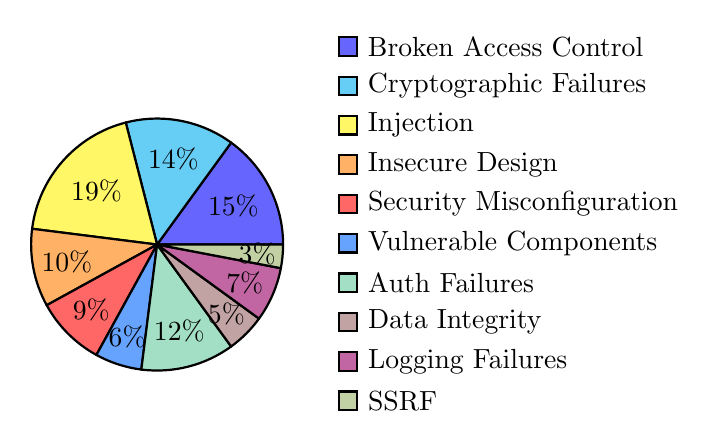
\begin{tikzpicture}[scale=0.8]
\pie[text=legend,radius=2]{
    15/Broken Access Control,
    14/Cryptographic Failures,
    19/Injection,
    10/Insecure Design,
    9/Security Misconfiguration,
    6/Vulnerable Components,
    12/Auth Failures,
    5/Data Integrity,
    7/Logging Failures,
    3/SSRF
}
\end{tikzpicture}
\end{columns}
\vspace{0.3cm}
\begin{center}
\textcolor{owaspyellow}{\textbf{Note:}} These risks are based on real-world data from thousands of applications and security assessments
\end{center}
\end{frame}

\begin{frame}[fragile]{A01:2021 - Broken Access Control}
\begin{columns}
\column{0.5\textwidth}
\textbf{What is Broken Access Control?}
\begin{itemize}
\item Users can access resources or perform actions beyond their intended permissions
\item Most common security vulnerability in web applications
\item Affects 94\% of applications tested
\item Can lead to data breaches and privilege escalation
\end{itemize}
\textbf{Common Attack Vectors:}
\begin{itemize}
\item[\faIcon{exclamation-triangle}] Insecure direct object references (IDOR)
\item[\faIcon{exclamation-triangle}] Missing access control checks
\item[\faIcon{exclamation-triangle}] Privilege escalation
\item[\faIcon{exclamation-triangle}]{Broken function level access control}
\end{itemize}
\column{0.5\textwidth}
\textbf{Vulnerable Code Example:}
\begin{lstlisting}[language=JavaScript]
// Vulnerable: No access control check
app.get('/api/users/:id', (req, res) => {
    const userId = req.params.id;
    const user = db.getUserById(userId);
    res.json(user); // Any user can access any user data
});

// Vulnerable: Parameter tampering
app.post('/api/admin/delete-user', (req, res) => {
    const userId = req.body.userId;
    db.deleteUser(userId); // No admin check
    res.json({ success: true });
});
\end{lstlisting}
\end{columns}
\end{frame}

\begin{frame}[fragile]{A01:2021 - Broken Access Control: Mitigation}
\begin{columns}
\column{0.5\textwidth}
\textbf{Secure Implementation:}
\begin{lstlisting}[language=JavaScript]
// Secure: Role-based access control
app.get('/api/users/:id', 
  requireAuth,
  requireRole(['admin', 'user']),
  (req, res) => {
    const userId = req.params.id;
    
    // Check if user can access this resource
    if (req.user.role !== 'admin' && 
        req.user.id !== userId) {
      return res.status(403).json({ 
        error: 'Access denied' 
      });
    }
    
    const user = db.getUserById(userId);
    res.json(user);
});

// Secure: Input validation and authorization
app.post('/api/admin/delete-user',
  requireAuth,
  requireRole(['admin']),
  validateInput,
  (req, res) => {
    const userId = req.body.userId;
    
    // Additional validation
    if (!isValidUserId(userId)) {
      return res.status(400).json({ 
        error: 'Invalid user ID' 
      });
    }
    
    db.deleteUser(userId);
    res.json({ success: true });
});
\end{lstlisting}
\column{0.5\textwidth}
\textbf{Best Practices:}
\begin{enumerate}
\item \textbf{Implement Access Control}
\begin{itemize}
\item[\faIcon{check}] Role-based access control (RBAC)
\item[\faIcon{check}] Attribute-based access control (ABAC)
\item[\faIcon{check}] Principle of least privilege
\end{itemize}
\item \textbf{Secure by Default}
\begin{itemize}
\item[\faIcon{check}] Default deny approach
\item[\faIcon{check}] Explicit allow lists
\item[\faIcon{check}] Fail secure mechanisms
\end{itemize}
\item \textbf{Regular Testing}
\begin{itemize}
\item[\faIcon{check}] Automated access control testing
\item[\faIcon{check}] Manual penetration testing
\item[\faIcon{check}] Regular access reviews
\end{itemize}
\item \textbf{Monitoring and Logging}
\begin{itemize}
\item[\faIcon{check}] Access violation logging
\item[\faIcon{check}] Anomaly detection
\item[\faIcon{check}] Alerting on suspicious access
\end{itemize}
\end{enumerate}
\end{columns}
\end{frame}

\begin{frame}[fragile]{A02:2021 - Cryptographic Failures}
\begin{columns}
\column{0.5\textwidth}
\textbf{What are Cryptographic Failures?}
\begin{itemize}
\item Sensitive data exposure due to weak cryptography
\item Affects 44\% of applications tested
\item Can lead to identity theft, financial loss, and data breaches
\end{itemize}
\textbf{Common Issues:}
\begin{itemize}
\item[\faIcon{exclamation-triangle}] Weak or broken encryption algorithms
\item[\faIcon{exclamation-triangle}] Hardcoded cryptographic keys
\item[\faIcon{exclamation-triangle}] Insecure storage of sensitive data
\item[\faIcon{exclamation-triangle}]{Missing or weak transport layer security}
\end{itemize}
\column{0.5\textwidth}
\textbf{Vulnerable Code Example:}
\begin{lstlisting}[language=JavaScript]
// Vulnerable: Weak hashing algorithm
const bcrypt = require('bcrypt');
const password = 'user123';

// Weak: Using MD5 (deprecated)
const weakHash = require('crypto')
  .createHash('md5')
  .update(password)
  .digest('hex');

// Vulnerable: Hardcoded encryption key
const crypto = require('crypto');
const algorithm = 'aes-256-cbc';
const key = 'ThisIsAHardcodedKey123'; // Never do this!
const iv = crypto.randomBytes(16);

function encrypt(text) {
  let cipher = crypto.createCipheriv(algorithm, key, iv);
  let encrypted = cipher.update(text, 'utf8', 'hex');
  encrypted += cipher.final('hex');
  return encrypted;
}
\end{lstlisting}
\end{columns}
\end{frame}

\begin{frame}[fragile]{A02:2021 - Cryptographic Failures: Mitigation}
\begin{columns}
\column{0.5\textwidth}
\textbf{Secure Implementation:}
\begin{lstlisting}[language=JavaScript]
// Secure: Strong password hashing
const bcrypt = require('bcrypt');
const password = 'user123';

// Strong: Using bcrypt with appropriate cost factor
const saltRounds = 12;
const strongHash = bcrypt.hashSync(password, saltRounds);

// Secure: Proper key management
const crypto = require('crypto');
const algorithm = 'aes-256-gcm';
const keyLength = 32; // 256 bits
const ivLength = 16; // 128 bits

// Generate secure key from environment variable
const key = crypto.scryptSync(
  process.env.ENCRYPTION_PASSWORD,
  process.env.ENCRYPTION_SALT,
  keyLength
);

function encrypt(text) {
  const iv = crypto.randomBytes(ivLength);
  const cipher = crypto.createCipheriv(algorithm, key, iv);
  
  let encrypted = cipher.update(text, 'utf8', 'hex');
  encrypted += cipher.final('hex');
  
  const authTag = cipher.getAuthTag();
  
  return {
    encrypted,
    iv: iv.toString('hex'),
    authTag: authTag.toString('hex')
  };
}

// Secure: Secure comparison to prevent timing attacks
function secureCompare(a, b) {
  if (typeof a !== 'string' || typeof b !== 'string') {
    return false;
  }
  
  const bufA = Buffer.from(a);
  const bufB = Buffer.from(b);
  
  if (bufA.length !== bufB.length) {
    return false;
  }
  
  return crypto.timingSafeEqual(bufA, bufB);
}
\end{lstlisting}
\column{0.5\textwidth}
\textbf{Best Practices:}
\begin{enumerate}
\item \textbf{Use Strong Algorithms}
\begin{itemize}
\item[\faIcon{check}] AES-256 for encryption
\item[\faIcon{check}] SHA-256/SHA-3 for hashing
\item[\faIcon{check}] RSA-2048+ for asymmetric crypto
\item[\faIcon{check}]{Elliptic curve cryptography}
\end{itemize}
\item \textbf{Proper Key Management}
\begin{itemize}
\item[\faIcon{check}] Use hardware security modules (HSM)
\item[\faIcon{check}] Implement key rotation
\item[\faIcon{check}] Store keys securely
\item[\faIcon{check}]{Use environment variables}
\end{itemize}
\item \textbf{Transport Security}
\begin{itemize}
\item[\faIcon{check}] TLS 1.2+ for all communications
\item[\faIcon{check}] Certificate pinning
\item[\faIcon{check}] HSTS headers
\item[\faIcon{check}]{Perfect forward secrecy}
\end{itemize}
\item \textbf{Data Protection}
\begin{itemize}
\item[\faIcon{check}] Encrypt sensitive data at rest
\item[\faIcon{check}] Use secure storage solutions
\item[\faIcon{check}] Implement data masking
\item[\faIcon{check}]{Regular security audits}
\end{itemize}
\end{enumerate}
\end{columns}
\end{frame}

\begin{frame}[fragile]{A03:2021 - Injection}
\begin{columns}
\column{0.5\textwidth}
\textbf{What is Injection?}
\begin{itemize}
\item Attackers can inject malicious code or commands into applications
\item Affects 33\% of applications tested
\item Can lead to data theft, data loss, and server takeover
\end{itemize}
\textbf{Common Injection Types:}
\begin{itemize}
\item[\faIcon{exclamation-triangle}] SQL Injection
\item[\faIcon{exclamation-triangle}] NoSQL Injection
\item[\faIcon{exclamation-triangle}] Command Injection
\item[\faIcon{exclamation-triangle}] LDAP Injection
\item[\faIcon{exclamation-triangle}]{XPath Injection}
\end{itemize}
\column{0.5\textwidth}
\textbf{Vulnerable Code Example:}
\begin{lstlisting}[language=JavaScript]
// Vulnerable: SQL Injection
app.get('/api/user/:id', (req, res) => {
    const userId = req.params.id;
    const query = `SELECT * FROM users WHERE id = ${userId}`;
    db.query(query, (err, results) => {
        res.json(results);
    });
});

// Vulnerable: Command Injection
app.post('/api/download', (req, res) => {
    const filename = req.body.filename;
    const command = `tar -czf backup.tar.gz ${filename}`;
    require('child_process').exec(command, (error, stdout, stderr) => {
        if (error) {
            res.status(500).send('Error');
        } else {
            res.send('Backup created');
        }
    });
});

// Vulnerable: NoSQL Injection
app.get('/api/search', (req, res) => {
    const username = req.query.username;
    const query = { username: username };
    db.users.findOne(query, (err, user) => {
        res.json(user);
    });
});
\end{lstlisting}
\end{columns}
\end{frame}

\begin{frame}[fragile]{A03:2021 - Injection: Mitigation}
\begin{columns}
\column{0.5\textwidth}
\textbf{Secure Implementation:}
\begin{lstlisting}[language=JavaScript]
// Secure: Parameterized queries (SQL)
const mysql = require('mysql2/promise');

app.get('/api/user/:id', async (req, res) => {
    const userId = req.params.id;
    
    try {
        const [rows] = await db.execute(
            'SELECT * FROM users WHERE id = ?',
            [userId] // Parameterized query
        );
        res.json(rows);
    } catch (error) {
        res.status(500).json({ error: 'Database error' });
    }
});

// Secure: Input validation and sanitization
const { body, validationResult } = require('express-validator');

app.post('/api/download', [
    body('filename')
        .isLength({ min: 1, max: 100 })
        .matches(/^[a-zA-Z0-9._-]+$/)
        .withMessage('Invalid filename')
], (req, res) => {
    const errors = validationResult(req);
    if (!errors.isEmpty()) {
        return res.status(400).json({ errors: errors.array() });
    }
    
    const filename = req.body.filename;
    const safeFilename = path.basename(filename);
    const command = `tar -czf backup.tar.gz "${safeFilename}"`;
    
    // Use safe execution with proper error handling
    require('child_process').exec(command, (error, stdout, stderr) => {
        if (error) {
            res.status(500).send('Error creating backup');
        } else {
            res.send('Backup created successfully');
        }
    });
});

// Secure: NoSQL with proper escaping
const { MongoClient } = require('mongodb');

app.get('/api/search', async (req, res) => {
    const username = req.query.username;
    
    try {
        const client = await MongoClient.connect(process.env.MONGODB_URI);
        const db = client.db();
        
        // Use parameterized query for NoSQL
        const user = await db.collection('users').findOne({
            username: { $eq: username }
        });
        
        res.json(user);
        client.close();
    } catch (error) {
        res.status(500).json({ error: 'Database error' });
    }
});
\end{lstlisting}
\column{0.5\textwidth}
\textbf{Best Practices:}
\begin{enumerate}
\item \textbf{Use Prepared Statements}
\begin{itemize}
\item[\faIcon{check}] Parameterized queries for SQL
\item[\faIcon{check}]{ORM with proper escaping}
\item[\faIcon{check}]{Stored procedures with proper permissions}
\item[\faIcon{check}]{Input validation frameworks}
\end{itemize}
\item \textbf{Input Validation}
\begin{itemize}
\item[\faIcon{check}]{Whitelist approach}
\item[\faIcon{check}]{Input length restrictions}
\item[\faIcon{check}]{Type checking}
\item[\faIcon{check}]{Regular expression validation}
\end{itemize}
\item \textbf{Output Encoding}
\begin{itemize}
\item[\faIcon{check}]{HTML encoding for web output}
\item[\faIcon{check}]{JavaScript encoding}
\item[\faIcon{check}]{URL encoding}
\item[\faIcon{check}]{Context-aware encoding}
\end{itemize}
\item \textbf{Security Controls}
\begin{itemize}
\item[\faIcon{check}]{Web Application Firewall (WAF)}
\item[\faIcon{check}]{Input sanitization libraries}
\item[\faIcon{check}]{Static Application Security Testing (SAST)}
\item[\faIcon{check}]{Dynamic Application Security Testing (DAST)}
\end{itemize}
\end{enumerate}
\end{columns}
\end{frame}

\begin{frame}[fragile]{A04:2021 - Insecure Design}
\begin{columns}
\column{0.5\textwidth}
\textbf{What is Insecure Design?}
\begin{itemize}
\item Security is not considered during the design phase
\item Results in fundamental security flaws that are difficult to fix
\item Affects 23\% of applications tested
\end{itemize}
\textbf{Common Design Flaws:}
\begin{itemize}
\item[\faIcon{exclamation-triangle}] Missing threat modeling
\item[\faIcon{exclamation-triangle}] Insecure data flow design
\item[\faIcon{exclamation-triangle}] Weak authentication flows
\item[\faIcon{exclamation-triangle}]{Lack of security by design}
\end{itemize}
\column{0.5\textwidth}
\textbf{Design Principles:}
\begin{enumerate}
\item \textbf{Zero Trust Architecture}
\begin{itemize}
\item Never trust, always verify
\item Micro-segmentation
\item Continuous authentication
\end{itemize}
\item \textbf{Defense in Depth}
\begin{itemize}
\item Multiple security layers
\item Redundant controls
\item Fail-safe mechanisms
\end{itemize}
\item \textbf{Security by Design}
\begin{itemize}
\item Threat modeling
\item Risk assessment
\item Secure coding standards
\end{itemize}
\item \textbf{Privacy by Design}
\begin{itemize}
\item Data minimization
\item Purpose limitation
\item User consent mechanisms
\end{itemize}
\end{enumerate}
\end{columns}
\end{frame}

\begin{frame}[fragile]{A04:2021 - Insecure Design: Mitigation}
\begin{columns}
\column{0.5\textwidth}
\textbf{Secure Design Patterns:}
\begin{lstlisting}[language=JavaScript]
// Secure: Authentication flow design
const express = require('express');
const session = require('express-session');
const crypto = require('crypto');

const app = express();

// Secure session configuration
app.use(session({
    secret: process.env.SESSION_SECRET,
    resave: false,
    saveUninitialized: false,
    cookie: {
        secure: true, // HTTPS only
        httpOnly: true, // JavaScript access
        maxAge: 24 * 60 * 60 * 1000, // 24 hours
        sameSite: 'strict' // CSRF protection
    }
}));

// Secure: Multi-factor authentication flow
app.post('/api/login', async (req, res) => {
    const { username, password, totpToken } = req.body;
    
    try {
        // Step 1: Verify credentials
        const user = await authenticateUser(username, password);
        
        // Step 2: Verify TOTP
        if (!verifyTOTP(user.totpSecret, totpToken)) {
            return res.status(401).json({ error: 'Invalid TOTP' });
        }
        
        // Step 3: Generate secure session
        const sessionId = crypto.randomBytes(32).toString('hex');
        req.session.user = {
            id: user.id,
            username: user.username,
            role: user.role
        };
        
        // Step 4: Log successful login
        await logSecurityEvent('login_success', user.id);
        
        res.json({ success: true });
    } catch (error) {
        // Step 5: Log failed login attempt
        await logSecurityEvent('login_failure', username);
        res.status(401).json({ error: 'Authentication failed' });
    }
});

// Secure: Rate limiting design
const rateLimit = require('express-rate-limit');

const loginLimiter = rateLimit({
    windowMs: 15 * 60 * 1000, // 15 minutes
    max: 5, // limit each IP to 5 login requests per window
    message: 'Too many login attempts, please try again later',
    standardHeaders: true,
    legacyHeaders: false,
});

app.post('/api/login', loginLimiter, (req, res) => {
    // Login logic with rate limiting
});
\end{lstlisting}
\column{0.5\textwidth}
\textbf{Design Methodologies:}
\begin{enumerate}
\item \textbf{Threat Modeling}
\begin{itemize}
\item[\faIcon{check}] STRIDE methodology
\item[\faIcon{check}] Attack surface analysis
\item[\faIcon{check}] Risk assessment matrix
\item[\faIcon{check}] Mitigation strategies
\end{itemize}
\item \textbf{Secure Architecture Patterns}
\begin{itemize}
\item[\faIcon{check}] Gateway pattern
\item[\faIcon{check}] Circuit breaker pattern
\item[\faIcon{check}] Observer pattern
\item[\faIcon{check}] Decorator pattern
\end{itemize}
\item \textbf{Security Requirements}
\begin{itemize}
\item[\faIcon{check}] Non-functional security requirements
\item[\faIcon{check}] Acceptance criteria
\item[\faIcon{check}] Compliance requirements
\item[\faIcon{check}] Performance impact analysis
\end{itemize}
\item \textbf{Design Reviews}
\begin{itemize}
\item[\faIcon{check}] Security design reviews
\item[\faIcon{check}] Peer reviews
\item[\faIcon{check}] Third-party assessments
\item[\faIcon{check}] Continuous improvement
\end{itemize}
\end{enumerate}
\end{columns}
\end{frame}

\begin{frame}[fragile]{A05:2021 - Security Misconfiguration}
\begin{columns}
\column{0.5\textwidth}
\textbf{What is Security Misconfiguration?}
\begin{itemize}
\item Security settings are not properly implemented or maintained
\item Affects 19\% of applications tested
\item Often due to lack of security knowledge or oversight
\end{itemize}
\textbf{Common Misconfigurations:}
\begin{itemize}
\item[\faIcon{exclamation-triangle}] Default credentials
\item[\faIcon{exclamation-triangle}] Verbose error messages
\item[\faIcon{exclamation-triangle}] Unnecessary services enabled
\item[\faIcon{exclamation-triangle}]{Missing security headers}
\end{itemize}
\column{0.5\textwidth}
\textbf{Vulnerable Configuration:}
\begin{lstlisting}
# Vulnerable: Nginx misconfiguration
server {
    listen 80;
    server_name example.com;
    
    # Missing security headers
    # Missing SSL/TLS configuration
    # Default directory listing enabled
    autoindex on;
    
    # Verbose error messages
    error_page 404 /404.html;
    error_page 500 /500.html;
    
    # Weak file permissions
    location / {
        root /var/www/html;
        index index.html;
        # Missing access controls
    }
}

# Vulnerable: Database configuration
[mysqld]
# Default root password
skip-grant-tables
# Network accessible
bind-address = 0.0.0.0
# Logging disabled
general_log = 0
# Insecure file privileges
secure-file-priv = /
\end{lstlisting}
\end{columns}
\end{frame}

\begin{frame}[fragile]{A05:2021 - Security Misconfiguration: Mitigation}
\begin{columns}
\column{0.5\textwidth}
\textbf{Secure Configuration:}
\begin{lstlisting}
# Secure: Nginx configuration
server {
    listen 443 ssl http2;
    server_name example.com;
    
    # SSL/TLS configuration
    ssl_certificate /etc/ssl/certs/cert.pem;
    ssl_certificate_key /etc/ssl/private/key.pem;
    ssl_protocols TLSv1.2 TLSv1.3;
    ssl_ciphers HIGH:!aNULL:!MD5:!RC4;
    ssl_prefer_server_ciphers on;
    
    # Security headers
    add_header X-Frame-Options "SAMEORIGIN" always;
    add_header X-Content-Type-Options "nosniff" always;
    add_header X-XSS-Protection "1; mode=block" always;
    add_header Strict-Transport-Security "max-age=31536000; includeSubDomains" always;
    add_header Content-Security-Policy "default-src 'self'; script-src 'self' 'unsafe-inline'; style-src 'self' 'unsafe-inline'" always;
    
    # Secure file serving
    location / {
        root /var/www/html;
        index index.html;
        try_files $uri $uri/ =404;
        autoindex off;
    }
    
    # Block access to sensitive files
    location ~* \.(env|log|conf|htaccess)$ {
        deny all;
        return 404;
    }
    
    # Rate limiting
    limit_req_zone $binary_remote_addr zone=api:10m rate=10r/s;
    location /api/ {
        limit_req zone=api burst=20 nodelay;
    }
}

# Secure: Database configuration
[mysqld]
# Remove default privileges
skip-grant-tables=0

# Secure network access
bind-address = 127.0.0.1

# Enable logging
general_log = 1
general_log_file = /var/log/mysql/mysql.log

# Secure file privileges
secure-file-priv = /var/lib/mysql/secure-files

# Enable SSL
ssl-ca = /etc/ssl/certs/ca.pem
ssl-cert = /etc/ssl/certs/server-cert.pem
ssl-key = /etc/ssl/private/server-key.pem
\end{lstlisting}
\column{0.5\textwidth}
\textbf{Configuration Management:}
\begin{enumerate}
\item \textbf{Secure Deployment}
\begin{itemize}
\item[\faIcon{check}] Infrastructure as Code (IaC)
\item[\faIcon{check}] Configuration templates
\item[\faIcon{check}] Automated deployment pipelines
\item[\faIcon{check}]{Configuration validation}
\end{itemize}
\item \textbf{Regular Audits}
\begin{itemize}
\item[\faIcon{check}] Configuration scanning
\item[\faIcon{check}] Compliance checks
\item[\faIcon{check}] Security assessments
\item[\faIcon{check}]{Vulnerability scanning}
\end{itemize}
\item \textbf{Change Management}
\begin{itemize}
\item[\faIcon{check}] Version control for configs
\item[\faIcon{check}] Change approval process
\item[\faIcon{check}] Rollback procedures
\item[\faIcon{check}]{Testing before deployment}
\end{itemize}
\item \textbf{Monitoring and Alerting}
\begin{itemize}
\item[\faIcon{check}] Configuration drift detection
\item[\faIcon{check}] Unauthorized change alerts
\item[\faIcon{check}] Compliance monitoring
\item[\faIcon{check}]{Performance impact analysis}
\end{itemize}
\end{enumerate}
\end{columns}
\end{frame}

\begin{frame}[fragile]{A06:2021 - Vulnerable and Outdated Components}
\begin{columns}
\column{0.5\textwidth}
\textbf{What are Vulnerable Components?}
\begin{itemize}
\item Using third-party libraries with known vulnerabilities
\item Affects 17\% of applications tested
\item Can lead to complete system compromise
\end{itemize}
\textbf{Common Issues:}
\begin{itemize}
\item[\faIcon{exclamation-triangle}] Known CVEs in dependencies
\item[\faIcon{exclamation-triangle}] Outdated software versions
\item[\faIcon{exclamation-triangle}] Unmanaged dependencies
\item[\faIcon{exclamation-triangle}]{Lack of dependency scanning}
\end{itemize}
\column{0.5\textwidth}
\textbf{Vulnerable Dependencies:}
\begin{lstlisting}[language=JavaScript]
// package.json with vulnerable dependencies
{
  "name": "vulnerable-app",
  "version": "1.0.0",
  "dependencies": {
    "express": "4.16.0", // vulnerable to multiple CVEs
    "lodash": "4.17.11", // prototype pollution vulnerability
    "moment": "2.22.2", // prototype pollution vulnerability
    "ws": "6.2.1", // vulnerable to WebSocket attacks
    "mysql": "2.16.0" // vulnerable to SQL injection
  },
  "devDependencies": {
    "nodemon": "1.18.9", // vulnerable to path traversal
    "jest": "23.6.0" // vulnerable to prototype pollution
  }
}

// Vulnerable: Using deprecated functions
const vulnerableFunction = require('vulnerable-lib');
const result = vulnerableFunction.processData(userInput);
\end{lstlisting}
\end{columns}
\end{frame}

\begin{frame}[fragile]{A06:2021 - Vulnerable Components: Mitigation}
\begin{columns}
\column{0.5\textwidth}
\textbf{Secure Dependency Management:}
\begin{lstlisting}[language=JavaScript]
// package.json with secure dependencies
{
  "name": "secure-app",
  "version": "1.0.0",
  "dependencies": {
    "express": "^4.18.2", // latest secure version
    "lodash": "^4.17.21", // patched version
    "moment": "^2.29.4", // patched version
    "ws": "^8.13.0", // latest secure version
    "mysql2": "^3.6.0" // secure MySQL driver
  },
  "devDependencies": {
    "nodemon": "^3.0.1", // latest secure version
    "jest": "^29.5.0" // latest secure version
  },
  "engines": {
    "node": ">=16.0.0" // minimum Node.js version
  }
}

// Secure: Dependency scanning
const { execSync } = require('child_process');

// Run npm audit to check for vulnerabilities
function checkVulnerabilities() {
  try {
    const result = execSync('npm audit --audit-level moderate');
    console.log('Vulnerability scan result:', result.toString());
  } catch (error) {
    console.error('Vulnerabilities found:', error.message);
    // Handle vulnerabilities appropriately
  }
}

// Secure: Use secure alternatives
const crypto = require('crypto');
const bcrypt = require('bcrypt');

// Instead of vulnerable crypto functions
function secureHash(data) {
  return crypto.createHash('sha256').update(data).digest('hex');
}

// Instead of weak password hashing
async function securePasswordHash(password) {
  const salt = await bcrypt.genSalt(12);
  return await bcrypt.hash(password, salt);
}
\end{lstlisting}
\column{0.5\textwidth}
\textbf{Dependency Management Best Practices:}
\begin{enumerate}
\item \textbf{Dependency Scanning}
\begin{itemize}
\item[\faIcon{check}] npm audit, Snyk, Dependabot
\item[\faIcon{check}]{OWASP Dependency Check}
\item[\faIcon{check}]{GitHub Dependabot alerts}
\item[\faIcon{check}]{Automated CI/CD scanning}
\end{itemize}
\item \textbf{Version Management}
\begin{itemize}
\item[\faIcon{check}]{Use caret (\textasciicircum) or tilde (\textasciitilde) operators}
\item[\faIcon{check}]{Regular updates testing}
\item[\faIcon{check}]{Semantic versioning}
\item[\faIcon{check}]{Patch management process}
\end{itemize}
\item \textbf{Secure Alternatives}
\begin{itemize}
\item[\faIcon{check}]{Use secure libraries}
\item[\faIcon{check}]{Avoid deprecated functions}
\item[\faIcon{check}]{Implement custom security}
\item[\faIcon{check}]{Code review of dependencies}
\end{itemize}
\item \textbf{Monitoring and Updates}
\begin{itemize}
\item[\faIcon{check}]{CVE monitoring}
\item[\faIcon{check}]{Security newsletters}
\item[\faIcon{check}]{Vendor security alerts}
\item[\faIcon{check}]{Regular update schedule}
\end{itemize}
\end{enumerate}
\end{columns}
\end{frame}

\begin{frame}[fragile]{A07:2021 - Identification and Authentication Failures}
\begin{columns}
\column{0.5\textwidth}
\textbf{What are Authentication Failures?}
\begin{itemize}
\item Identity verification and session management issues
\item Affects 13\% of applications tested
\item Can lead to account takeover and unauthorized access
\end{itemize}
\textbf{Common Issues:}
\begin{itemize}
\item[\faIcon{exclamation-triangle}] Weak password policies
\item[\faIcon{exclamation-triangle}] Insecure session management
\item[\faIcon{exclamation-triangle}] Missing multi-factor authentication
\item[\faIcon{exclamation-triangle}]{Credential stuffing attacks}
\end{itemize}
\column{0.5\textwidth}
\textbf{Vulnerable Authentication:}
\begin{lstlisting}[language=JavaScript]
// Vulnerable: Weak password hashing
const crypto = require('crypto');

function hashPassword(password) {
  // Weak: Using MD5 (deprecated)
  return crypto.createHash('md5').update(password).digest('hex');
}

// Vulnerable: Insecure session management
const express = require('express');
const session = require('express-session');

const app = express();

// Insecure: Default session configuration
app.use(session({
  secret: 'weak-secret-key',
  resave: true,
  saveUninitialized: true,
  cookie: {
    secure: false, // HTTP allowed
    httpOnly: false, // JavaScript accessible
    maxAge: 86400000 // 24 hours
  }
}));

// Vulnerable: No rate limiting on login
app.post('/api/login', (req, res) => {
  const { username, password } = req.body;
  
  // No input validation
  const user = db.getUser(username, password);
  
  if (user) {
    req.session.user = user;
    res.json({ success: true });
  } else {
    res.status(401).json({ error: 'Invalid credentials' });
  }
});
\end{lstlisting}
\end{columns}
\end{frame}

\begin{frame}[fragile]{A07:2021 - Authentication Failures: Mitigation}
\begin{columns}
\column{0.5\textwidth}
\textbf{Secure Authentication:}
\begin{lstlisting}[language=JavaScript]
// Secure: Strong password hashing
const bcrypt = require('bcrypt');

async function hashPassword(password) {
  // Strong: Using bcrypt with appropriate cost factor
  const saltRounds = 12;
  return await bcrypt.hash(password, saltRounds);
}

// Secure: Secure session management
const express = require('express');
const session = require('express-session');
const crypto = require('crypto');

const app = express();

// Secure: Enhanced session configuration
app.use(session({
  secret: process.env.SESSION_SECRET,
  resave: false,
  saveUninitialized: false,
  store: new session.MemoryStore(),
  cookie: {
    secure: true, // HTTPS only
    httpOnly: true, // JavaScript inaccessible
    maxAge: 3600000, // 1 hour
    sameSite: 'strict' // CSRF protection
  }
}));

// Secure: Rate-limited login with MFA
const rateLimit = require('express-rate-limit');

const loginLimiter = rateLimit({
  windowMs: 15 * 60 * 1000, // 15 minutes
  max: 5, // limit each IP to 5 login attempts
  message: 'Too many login attempts'
});

app.post('/api/login', loginLimiter, async (req, res) => {
  const { username, password, totpToken } = req.body;
  
  try {
    // Input validation
    if (!username || !password) {
      return res.status(400).json({ error: 'Username and password required' });
    }
    
    // Verify credentials
    const user = await authenticateUser(username, password);
    
    if (!user) {
      // Log failed attempt
      await logFailedLogin(username, req.ip);
      return res.status(401).json({ error: 'Invalid credentials' });
    }
    
    // Verify MFA
    if (user.mfaEnabled && !verifyTOTP(user.totpSecret, totpToken)) {
      return res.status(401).json({ error: 'Invalid MFA token' });
    }
    
    // Generate secure session
    const sessionId = crypto.randomBytes(32).toString('hex');
    req.session.regenerate((err) => {
      if (err) {
        return res.status(500).json({ error: 'Session error' });
      }
      
      req.session.user = {
        id: user.id,
        username: user.username,
        role: user.role
      };
      
      // Log successful login
      await logSuccessfulLogin(user.id, req.ip);
      
      res.json({ success: true });
    });
  } catch (error) {
    res.status(500).json({ error: 'Authentication error' });
  }
});
\end{lstlisting}
\column{0.5\textwidth}
\textbf{Authentication Best Practices:}
\begin{enumerate}
\item \textbf{Strong Password Policies}
\begin{itemize}
\item[\faIcon{check}] Minimum 12 characters
\item[\faIcon{check}]{Complexity requirements}
\item[\faIcon{check}]{Password rotation}
\item[\faIcon{check}]{Password blacklist}
\end{itemize}
\item \textbf{Multi-Factor Authentication}
\begin{itemize}
\item[\faIcon{check}]{TOTP (Google Authenticator)}
\item[\faIcon{check}]{SMS/Email verification}
\item[\faIcon{check}]{Hardware tokens}
\item[\faIcon{check}]{Biometric authentication}
\end{itemize}
\item \textbf{Session Security}
\begin{itemize}
\item[\faIcon{check}]{Secure session cookies}
\item[\faIcon{check}]{Session timeout}
\item[\faIcon{check}]{Session invalidation}
\item[\faIcon{check}]{CSRF protection}
\end{itemize}
\item \textbf{Account Protection}
\begin{itemize}
\item[\faIcon{check}]{Account lockout policies}
\item[\faIcon{check}]{Brute force protection}
\item[\faIcon{check}]{Suspicious activity monitoring}
\item[\faIcon{check}]{Passwordless authentication}
\end{itemize}
\end{enumerate}
\end{columns}
\end{frame}

\begin{frame}[fragile]{A08:2021 - Software and Data Integrity Failures}
\begin{columns}
\column{0.5\textwidth}
\textbf{What are Integrity Failures?}
\begin{itemize}
\item Software and data can be modified or corrupted without detection
\item Affects 10\% of applications tested
\item Can lead to unauthorized changes and data corruption
\end{itemize}
\textbf{Common Issues:}
\begin{itemize}
\item[\faIcon{exclamation-triangle}] Insecure deserialization
\item[\faIcon{exclamation-triangle}] Missing integrity checks
\item[\faIcon{exclamation-triangle}] Unvalidated inputs
\item[\faIcon{exclamation-triangle}]{Missing digital signatures}
\end{itemize}
\column{0.5\textwidth}
\textbf{Vulnerable Code:}
\begin{lstlisting}[language=JavaScript]
// Vulnerable: Insecure deserialization
const { deserialize } = require('vulnerable-parser');

function processData(data) {
  // Dangerous: Direct deserialization without validation
  const obj = deserialize(data);
  return obj;
}

// Vulnerable: Missing integrity checks
const fs = require('fs');

function updateConfig(configPath, newConfig) {
  // No integrity check before writing
  fs.writeFileSync(configPath, JSON.stringify(newConfig));
}

// Vulnerable: Unvalidated file uploads
const multer = require('multer');

const upload = multer({ dest: 'uploads/' });

app.post('/api/upload', upload.single('file'), (req, res) => {
  const file = req.file;
  
  // No file type validation
  // No file size validation
  // No virus scanning
  
  // Move file to production directory
  const newPath = `./public/${file.originalname}`;
  fs.renameSync(file.path, newPath);
  
  res.json({ success: true, path: newPath });
});
\end{lstlisting}
\end{columns}
\end{frame}

\begin{frame}[fragile]{A08:2021 - Integrity Failures: Mitigation}
\begin{columns}
\column{0.5\textwidth}
\textbf{Secure Implementation:}
\begin{lstlisting}[language=JavaScript]
// Secure: Safe deserialization
const { safeDeserialize } = require('secure-parser');

function processData(data) {
  try {
    // Validate input before deserialization
    if (!isValidSerializedData(data)) {
      throw new Error('Invalid serialized data');
    }
    
    // Use safe deserialization
    const obj = safeDeserialize(data);
    
    // Validate deserialized object
    if (!isValidObject(obj)) {
      throw new Error('Invalid object structure');
    }
    
    return obj;
  } catch (error) {
    console.error('Deserialization error:', error);
    throw new Error('Data processing failed');
  }
}

// Secure: File integrity verification
const crypto = require('crypto');
const fs = require('fs');

function updateConfig(configPath, newConfig, expectedHash) {
  try {
    // Validate configuration structure
    if (!isValidConfig(newConfig)) {
      throw new Error('Invalid configuration');
    }
    
    // Calculate hash of new configuration
    const newHash = crypto.createHash('sha256')
      .update(JSON.stringify(newConfig))
      .digest('hex');
    
    // Verify integrity if hash provided
    if (expectedHash && newHash !== expectedHash) {
      throw new Error('Configuration integrity check failed');
    }
    
    // Create backup before update
    const backupPath = `${configPath}.backup.${Date.now()}`;
    if (fs.existsSync(configPath)) {
      fs.copyFileSync(configPath, backupPath);
    }
    
    // Write new configuration
    fs.writeFileSync(configPath, JSON.stringify(newConfig, null, 2));
    
    return { success: true, hash: newHash };
  } catch (error) {
    console.error('Config update error:', error);
    throw error;
  }
}

// Secure: File upload with validation
const multer = require('multer');
const path = require('path');

// Configure multer with security options
const upload = multer({
  dest: 'uploads/',
  limits: {
    fileSize: 5 * 1024 * 1024, // 5MB limit
  },
  fileFilter: (req, file, cb) => {
    // Allowed file types
    const allowedTypes = ['image/jpeg', 'image/png', 'application/pdf'];
    
    if (!allowedTypes.includes(file.mimetype)) {
      return cb(new Error('Invalid file type'), false);
    }
    
    // Check file extension
    const fileExtension = path.extname(file.originalname).toLowerCase();
    const allowedExtensions = ['.jpg', '.jpeg', '.png', '.pdf'];
    
    if (!allowedExtensions.includes(fileExtension)) {
      return cb(new Error('Invalid file extension'), false);
    }
    
    cb(null, true);
  }
});

app.post('/api/upload', upload.single('file'), (req, res) => {
  const file = req.file;
  
  try {
    // Generate secure filename
    const safeFilename = `${Date.now()}-${file.originalname}`;
    const newPath = `./public/${safeFilename}`;
    
    // Move file to secure location
    fs.renameSync(file.path, newPath);
    
    // Calculate file hash for integrity
    const fileHash = crypto.createHash('sha256')
      .update(fs.readFileSync(newPath))
      .digest('hex');
    
    res.json({
      success: true,
      path: newPath,
      filename: safeFilename,
      hash: fileHash,
      size: file.size
    });
  } catch (error) {
    res.status(500).json({ error: 'File upload failed' });
  }
});
\end{lstlisting}
\column{0.5\textwidth}
\textbf{Integrity Best Practices:}
\begin{enumerate}
\item \textbf{Input Validation}
\begin{itemize}
\item[\faIcon{check}]{Strict input validation}
\item[\faIcon{check}]{Type checking}
\item[\faIcon{check}]{Length restrictions}
\item[\faIcon{check}]{Format validation}
\end{itemize}
\item \textbf{Secure Deserialization}
\begin{itemize}
\item[\faIcon{check}]{Use safe parsers}
\item[\faIcon{check}]{Validate before deserialization}
\item[\faIcon{check}]{Implement sandboxing}
\item[\faIcon{check}]{Use JSON instead of binary formats}
\end{itemize}
\item \textbf{Data Integrity}
\begin{itemize}
\item[\faIcon{check}]{Cryptographic hashing}
\item[\faIcon{check}]{Digital signatures}
\item[\faIcon{check}]{Checksum verification}
\item[\faIcon{check}]{Version control}
\end{itemize}
\item \textbf{File Security}
\begin{itemize}
\item[\faIcon{check}]{File type validation}
\item[\faIcon{check}]{File size limits}
\item[\faIcon{check}]{Virus scanning}
\item[\faIcon{check}]{Secure file storage}
\end{itemize}
\end{enumerate}
\end{columns}
\end{frame}

\begin{frame}[fragile]{A09:2021 - Security Logging and Monitoring Failures}
\begin{columns}
\column{0.5\textwidth}
\textbf{What are Logging Failures?}
\begin{itemize}
\item Insufficient logging and monitoring allows attackers to go undetected
\item Affects 8\% of applications tested
\item Can lead to prolonged attacks and data breaches
\end{itemize}
\textbf{Common Issues:}
\begin{itemize}
\item[\faIcon{exclamation-triangle}] Insufficient logging
\item[\faIcon{exclamation-triangle}] Missing security events
\item[\faIcon{exclamation-triangle}] No monitoring or alerting
\item[\faIcon{exclamation-triangle}]{Insufficient log retention}
\end{itemize}
\column{0.5\textwidth}
\textbf{Vulnerable Logging:}
\begin{lstlisting}[language=JavaScript]
// Vulnerable: Insufficient logging
const express = require('express');
const app = express();

app.post('/api/login', (req, res) => {
  const { username, password } = req.body;
  
  // No logging of login attempts
  const user = db.getUser(username, password);
  
  if (user) {
    req.session.user = user;
    res.json({ success: true });
  } else {
    // No logging of failed attempts
    res.status(401).json({ error: 'Invalid credentials' });
  }
});

// Vulnerable: No security monitoring
app.get('/api/admin/users', (req, res) => {
  // No logging of admin access
  const users = db.getUsers();
  res.json(users);
});

// Vulnerable: Verbose error messages
app.get('/api/user/:id', (req, res) => {
  try {
    const user = db.getUserById(req.params.id);
    res.json(user);
  } catch (error) {
    // Information disclosure in error messages
    res.status(500).json({ 
      error: 'Database error: ' + error.message 
    });
  }
});
\end{lstlisting}
\end{columns}
\end{frame}

\begin{frame}[fragile]{A09:2021 - Logging Failures: Mitigation}
\begin{columns}
\column{0.5\textwidth}
\textbf{Secure Logging:}
\begin{lstlisting}[language=JavaScript]
// Secure: Comprehensive logging
const winston = require('winston');
const { combine, timestamp, printf } = winston.format;

// Custom log format
const logFormat = printf(({ level, message, timestamp }) => {
  return `${timestamp} [${level}]: ${message}`;
});

// Create logger instance
const logger = winston.createLogger({
  level: 'info',
  format: combine(
    timestamp(),
    logFormat
  ),
  transports: [
    new winston.transports.File({ 
      filename: 'logs/error.log', 
      level: 'error' 
    }),
    new winston.transports.File({ 
      filename: 'logs/combined.log' 
    }),
    new winston.transports.Console()
  ]
});

// Security event logger
const securityLogger = winston.createLogger({
  level: 'info',
  format: combine(
    timestamp(),
    logFormat
  ),
  transports: [
    new winston.transports.File({ 
      filename: 'logs/security.log' 
    })
  ]
});

// Secure: Login with comprehensive logging
app.post('/api/login', async (req, res) => {
  const { username, password } = req.body;
  const clientIp = req.ip;
  const userAgent = req.get('User-Agent');
  
  try {
    // Log login attempt
    logger.info('Login attempt', {
      username,
      ip: clientIp,
      userAgent,
      timestamp: new Date().toISOString()
    });
    
    const user = await authenticateUser(username, password);
    
    if (user) {
      // Log successful login
      securityLogger.info('Successful login', {
        userId: user.id,
        username: user.username,
        ip: clientIp,
        userAgent,
        timestamp: new Date().toISOString()
      });
      
      req.session.user = user;
      res.json({ success: true });
    } else {
      // Log failed login attempt
      securityLogger.warn('Failed login attempt', {
        username,
        ip: clientIp,
        userAgent,
        timestamp: new Date().toISOString()
      });
      
      res.status(401).json({ error: 'Invalid credentials' });
    }
  } catch (error) {
    logger.error('Login error', {
      error: error.message,
      stack: error.stack,
      timestamp: new Date().toISOString()
    });
    
    res.status(500).json({ error: 'Authentication error' });
  }
});

// Secure: Admin access logging
app.get('/api/admin/users', requireAuth, requireRole(['admin']), (req, res) => {
  const adminUser = req.session.user;
  
  // Log admin access
  securityLogger.info('Admin access', {
    adminId: adminUser.id,
    adminUsername: adminUser.username,
    action: 'view_users',
    timestamp: new Date().toISOString()
  });
  
  const users = db.getUsers();
  res.json(users);
});

// Secure: Error handling with appropriate logging
app.get('/api/user/:id', async (req, res) => {
  try {
    const user = await db.getUserById(req.params.id);
    res.json(user);
  } catch (error) {
    // Log error without exposing sensitive information
    logger.error('User retrieval error', {
      error: 'Failed to retrieve user',
      userId: req.params.id,
      timestamp: new Date().toISOString()
    });
    
    res.status(500).json({ error: 'Internal server error' });
  }
});
\end{lstlisting}
\column{0.5\textwidth}
\textbf{Logging Best Practices:}
\begin{enumerate}
\item \textbf{Comprehensive Logging}
\begin{itemize}
\item[\faIcon{check}]{Security events logging}
\item[\faIcon{check}]{Authentication events}
\item[\faIcon{check}]{Authorization events}
\item[\faIcon{check}]{Error events}
\end{itemize}
\item \textbf{Log Protection}
\begin{itemize}
\item[\faIcon{check}]{Secure log storage}
\item[\faIcon{check}]{Log access controls}
\item[\faIcon{check}]{Log tamper detection}
\item[\faIcon{check}]{Log encryption}
\end{itemize}
\item \textbf{Monitoring and Alerting}
\begin{itemize}
\item[\faIcon{check}]{Real-time monitoring}
\item[\faIcon{check}]{Anomaly detection}
\item[\faIcon{check}]{Alert thresholds}
\item[\faIcon{check}]{Automated responses}
\end{itemize}
\item \textbf{Log Management}
\begin{itemize}
\item[\faIcon{check}]{Log rotation}
\item[\faIcon{check}]{Log retention policies}
\item[\faIcon{check}]{Log aggregation}
\item[\faIcon{check}]{Log analysis tools}
\end{itemize}
\end{enumerate}
\end{columns}
\end{frame}

\begin{frame}[fragile]{A10:2021 - Server-Side Request Forgery (SSRF)}
\begin{columns}
\column{0.5\textwidth}
\textbf{What is SSRF?}
\begin{itemize}
\item Attackers can force the server to make requests to unintended locations
\item Affects 4\% of applications tested
\item Can lead to internal network access and data exfiltration
\end{itemize}
\textbf{Common Issues:}
\begin{itemize}
\item[\faIcon{exclamation-triangle}] User-controlled URLs
\item[\faIcon{exclamation-triangle}] Missing input validation
\item[\faIcon{exclamation-triangle}] No network restrictions
\item[\faIcon{exclamation-triangle}]{Missing request validation}
\end{itemize}
\column{0.5\textwidth}
\textbf{Vulnerable SSRF Code:}
\begin{lstlisting}[language=JavaScript]
// Vulnerable: User-controlled URL requests
const axios = require('axios');

app.get('/api/fetch-url', (req, res) => {
  const url = req.query.url;
  
  // Dangerous: Direct request to user-provided URL
  axios.get(url)
    .then(response => {
      res.json(response.data);
    })
    .catch(error => {
      res.status(500).json({ error: 'Request failed' });
    });
});

// Vulnerable: File download with SSRF
const request = require('request');

app.get('/api/download', (req, res) => {
  const fileUrl = req.query.url;
  
  // No validation of URL
  request(fileUrl).pipe(res);
});

// Vulnerable: API proxy
app.get('/api/proxy', (req, res) => {
  const targetUrl = req.query.target;
  
  // SSRF vulnerability in proxy
  const proxyRequest = request(targetUrl);
  proxyRequest.pipe(res);
});
\end{lstlisting}
\end{columns}
\end{frame}

\begin{frame}[fragile]{A10:2021 - SSRF: Mitigation}
\begin{columns}
\column{0.5\textwidth}
\textbf{Secure SSRF Prevention:}
\begin{lstlisting}[language=JavaScript]
// Secure: URL validation and restrictions
const axios = require('axios');
const url = require('url');
const { URL } = require('url');

// Allowed domains list
const ALLOWED_DOMAINS = [
  'api.example.com',
  'trusted-service.com',
  'internal-service.local'
];

// Validate URL against allowed domains
function isUrlAllowed(targetUrl) {
  try {
    const parsedUrl = new URL(targetUrl);
    
    // Check if protocol is secure
    if (parsedUrl.protocol !== 'https:' && parsedUrl.protocol !== 'http:') {
      return false;
    }
    
    // Check if domain is in allowed list
    return ALLOWED_DOMAINS.some(domain => 
      parsedUrl.hostname === domain || 
      parsedUrl.hostname.endsWith(`.${domain}`)
    );
  } catch (error) {
    return false;
  }
}

app.get('/api/fetch-url', (req, res) => {
  const url = req.query.url;
  
  // Validate URL before making request
  if (!url || !isUrlAllowed(url)) {
    return res.status(400).json({ error: 'Invalid URL' });
  }
  
  // Make request with additional security
  axios.get(url, {
    timeout: 5000, // 5 second timeout
    maxRedirects: 0, // Prevent redirects
    validateStatus: function (status) {
      return status >= 200 && status < 300; // Only accept 2xx status
    }
  })
  .then(response => {
    // Validate response content type
    const contentType = response.headers['content-type'];
    if (!contentType || !contentType.includes('application/json')) {
      throw new Error('Invalid content type');
    }
    
    res.json(response.data);
  })
  .catch(error => {
    res.status(500).json({ error: 'Request failed' });
  });
});

// Secure: File download with validation
const request = require('request');

app.get('/api/download', (req, res) => {
  const fileUrl = req.query.url;
  
  // Validate URL
  if (!fileUrl || !isUrlAllowed(fileUrl)) {
    return res.status(400).json({ error: 'Invalid URL' });
  }
  
  // Secure download with restrictions
  const downloadRequest = request({
    uri: fileUrl,
    timeout: 10000, // 10 second timeout
    followRedirect: false, // Prevent redirects
    headers: {
      'User-Agent': 'Secure-Downloader/1.0'
    }
  });
  
  downloadRequest.pipe(res);
});

// Secure: API proxy with restrictions
app.get('/api/proxy', (req, res) => {
  const targetUrl = req.query.target;
  
  // Validate target URL
  if (!targetUrl || !isUrlAllowed(targetUrl)) {
    return res.status(400).json({ error: 'Invalid target URL' });
  }
  
  // Create secure proxy request
  const proxyRequest = request({
    uri: targetUrl,
    method: req.method,
    headers: req.headers,
    body: req.body,
    timeout: 30000, // 30 second timeout
    followRedirect: false
  });
  
  proxyRequest.pipe(res);
});
\end{lstlisting}
\column{0.5\textwidth}
\textbf{SSRF Prevention Best Practices:}
\begin{enumerate}
\item \textbf{URL Validation}
\begin{itemize}
\item[\faIcon{check}]{Whitelist allowed domains}
\item[\faIcon{check}]{Validate URL format}
\item[\faIcon{check}]{Block IP addresses}
\item[\faIcon{check}]{Prevent localhost access}
\end{itemize}
\item \textbf{Network Restrictions}
\begin{itemize}
\item[\faIcon{check}]{Firewall rules}
\item[\faIcon{check}]{Network segmentation}
\item[\faIcon{check}]{Proxy restrictions}
\item[\faIcon{check}]{VPN limitations}
\end{itemize}
\item \textbf{Request Security}
\begin{itemize}
\item[\faIcon{check}]{Request timeouts}
\item[\faIcon{check}]{Redirect prevention}
\item[\faIcon{check}]{Content validation}
\item[\faIcon{check}]{Header sanitization}
\end{itemize}
\item \textbf{Monitoring and Detection}
\begin{itemize}
\item[\faIcon{check}]{Request logging}
\item[\faIcon{check}]{Anomaly detection}
\item[\faIcon{check}]{Alerting on suspicious requests}
\item[\faIcon{check}]{Regular security assessments}
\end{itemize}
\end{enumerate}
\end{columns}
\end{frame}

\begin{frame}{Hands-on Lab: Vulnerability Assessment and Mitigation}
\begin{columns}
\column{0.5\textwidth}
\textbf{Lab Objectives:}
\begin{itemize}
\item[\faIcon{bullseye}] Identify vulnerabilities in web applications
\item[\faIcon{search}] Assess risk levels of identified threats
\item[\faIcon{shield-alt}] Develop mitigation strategies
\item[\faIcon{clipboard-check}] Create security testing reports
\end{itemize}
\textbf{Lab Environment Setup:}
\begin{enumerate}
\item Install Docker and vulnerable applications
\item Set up security scanning tools
\item Configure logging and monitoring
\item Prepare test cases and payloads
\end{enumerate}
\textbf{Tools Required:}
\begin{itemize}
\item[\faIcon{tools}] OWASP ZAP for web app scanning
\item[\faIcon{tools}] Burp Suite for manual testing
\item[\faIcon{tools}] SQLMap for SQL injection testing
\item[\faIcon{tools}]{Nmap for network scanning}
\end{itemize}
\column{0.5\textwidth}
\textbf{Lab Tasks:}
\begin{enumerate}
\item \textbf{Vulnerability Scanning}
\begin{itemize}
\item Run automated vulnerability scans
\item Identify OWASP Top 10 vulnerabilities
\item Document findings with evidence
\item Prioritize risks based on impact
\end{itemize}
\item \textbf{Manual Testing}
\begin{itemize}
\item Perform penetration testing
\item Test for injection attacks
\item Verify access control issues
\item Test authentication bypasses
\end{itemize}
\item \textbf{Mitigation Implementation}
\begin{itemize}
\item Apply security patches
\item Implement input validation
\item Configure security headers
\item Set up monitoring and alerting
\end{itemize}
\item \textbf{Documentation}
\begin{itemize}
\item Create vulnerability reports
\item Develop remediation plans
\item Create security policies
\item Document lessons learned
\end{itemize}
\end{enumerate}
\end{columns}
\end{frame}

\begin{frame}[fragile]{Practical Example: Secure Web Application}
\begin{columns}
\column{0.5\textwidth}
\textbf{Secure Application Features:}
\begin{enumerate}
\item \textbf{Authentication and Authorization}
\begin{itemize}
\item[\faIcon{check}] Multi-factor authentication
\item[\faIcon{check}] Role-based access control
\item[\faIcon{check}] Secure session management
\item[\faIcon{check}]{Passwordless authentication}
\end{itemize}
\item \textbf{Input Validation}
\begin{itemize}
\item[\faIcon{check}]{Whitelist validation}
\item[\faIcon{check}]{Input sanitization}
\item[\faIcon{check}]{Type checking}
\item[\faIcon{check}]{Length restrictions}
\end{itemize}
\item \textbf{Security Headers}
\begin{itemize}
\item[\faIcon{check}]{Content Security Policy}
\item[\faIcon{check}]{Strict Transport Security}
\item[\faIcon{check}]{X-Frame-Options}
\item[\faIcon{check}]{X-Content-Type-Options}
\end{itemize}
\item \textbf{Monitoring and Logging}
\begin{itemize}
\item[\faIcon{check}]{Security event logging}
\item[\faIcon{check}]{Real-time monitoring}
\item[\faIcon{check}]{Alerting system}
\item[\faIcon{check}]{Log analysis}
\end{itemize}
\end{enumerate}
\column{0.5\textwidth}
\textbf{Docker Compose for Security Testing:}
\begin{lstlisting}
version: '3.8'

services:
  # Target application
  vulnerable-app:
    image: vulnerable-web-app:latest
    ports:
      - "8080:80"
    environment:
      - DB_HOST=postgres
      - REDIS_HOST=redis
    depends_on:
      - postgres
      - redis

  # Database
  postgres:
    image: postgres:13
    environment:
      POSTGRES_DB: webapp
      POSTGRES_USER: secure_user
      POSTGRES_PASSWORD: ${DB_PASSWORD}
    volumes:
      - postgres_data:/var/lib/postgresql/data

  # Cache
  redis:
    image: redis:alpine
    command: redis-server --requirepass ${REDIS_PASSWORD}

  # Security tools
  zap:
    image: owasp/zap2docker-stable
    command: zap-baseline.py -t http://vulnerable-app:8080
    depends_on:
      - vulnerable-app

  # Burp Suite
  burp:
    image: burp-suite:latest
    ports:
      - "8081:8080"
    volumes:
      - ./burp-config:/config

volumes:
  postgres_data:
\end{lstlisting}
\end{columns}
\end{frame}

\begin{frame}{Security Assessment Checklist}
\begin{columns}
\column{0.5\textwidth}
\textbf{OWASP Top 10 Assessment Checklist:}
\begin{enumerate}
\item \textbf{Broken Access Control}
\begin{itemize}
\item[\faIcon{check}] Role-based access implemented
\item[\faIcon{check}] Authorization checks enforced
\item[\faIcon{check}] Insecure direct object references prevented
\item[\faIcon{check}]{Access control tested}
\end{itemize}
\item \textbf{Cryptographic Failures}
\begin{itemize}
\item[\faIcon{check}] Strong encryption algorithms used
\item[\faIcon{check}]{Secure key management}
\item[\faIcon{check}]{Transport security implemented}
\item[\faIcon{check}]{Sensitive data protected}
\end{itemize}
\item \textbf{Injection}
\begin{itemize}
\item[\faIcon{check}]{Parameterized queries used}
\item[\faIcon{check}]{Input validation implemented}
\item[\faIcon{check}]{Output encoding applied}
\item[\faIcon{check}]{Injection testing performed}
\end{itemize}
\item \textbf{Insecure Design}
\begin{itemize}
\item[\faIcon{check}]{Threat modeling conducted}
\item[\faIcon{check}]{Security by design principles}
\item[\faIcon{check}]{Zero trust architecture}
\item[\faIcon{check}]{Secure design patterns}
\end{itemize}
\end{enumerate}
\column{0.5\textwidth}
\textbf{Security Configuration Checklist:}
\begin{enumerate}
\item \textbf{Security Misconfiguration}
\begin{itemize}
\item[\faIcon{check}]{Default credentials changed}
\item[\faIcon{check}]{Security headers configured}
\item[\faIcon{check}]{Error messages secured}
\item[\faIcon{check}]{Services properly configured}
\end{itemize}
\item \textbf{Vulnerable Components}
\begin{itemize}
\item[\faIcon{check}]{Dependencies scanned}
\item[\faIcon{check}]{Known vulnerabilities patched}
\item[\faIcon{check}]{Outdated components updated}
\item[\faIcon{check}]{Secure alternatives used}
\end{itemize}
\item \textbf{Authentication Failures}
\begin{itemize}
\item[\faIcon{check}]{Strong password policies}
\item[\faIcon{check}]{Multi-factor authentication}
\item[\faIcon{check}]{Secure session management}
\item[\faIcon{check}]{Account protection measures}
\end{itemize}
\item \textbf{Logging and Monitoring}
\begin{itemize}
\item[\faIcon{check}]{Security events logged}
\item[\faIcon{check}]{Monitoring implemented}
\item[\faIcon{check}]{Alerting configured}
\item[\faIcon{check}]{Log retention policies}
\end{itemize}
\end{enumerate}
\end{columns}
\end{frame}

\begin{frame}{Summary and Key Takeaways}
\begin{columns}
\column{0.5\textwidth}
\textbf{OWASP Top 10 Fundamentals:}
\begin{itemize}
\item[\faIcon{shield-alt}] Understanding security risks
\item[\faIcon{search}] Identifying vulnerabilities
\item[\faIcon{tools}] Applying mitigation strategies
\item[\faIcon{clipboard-check}]{Implementing security controls}
\end{itemize}
\textbf{Security Best Practices:}
\begin{itemize}
\item[\faIcon{check-circle}] Defense in depth
\item[\faIcon{check-circle}]{Principle of least privilege}
\item[\faIcon{check-circle}]{Security by design}
\item[\faIcon{check-circle}]{Continuous security testing}
\end{itemize}
\column{0.5\textwidth}
\textbf{Practical Implementation:}
\begin{itemize}
\item[\faIcon{code}] Secure coding practices
\item[\faIcon{tools}]{Security tool integration}
\item[\faIcon{clipboard-check}]{Regular security assessments}
\item[\faIcon{book}]{Documentation and policies}
\end{itemize}
\textbf{Next Steps:}
\begin{itemize}
\item[\faIcon{arrow-right}] Apply concepts to real projects
\item[\faIcon{arrow-right}] Conduct security audits
\item[\faIcon{arrow-right}] Implement security controls
\item[\faIcon{arrow-right}]{Continuous improvement}
\end{itemize}
\end{columns}
\vspace{0.5cm}
\begin{center}
\Large{\textbf{Questions?}}\\
\vspace{0.3cm}
\normalsize{Contact: security-team@organization.com}\\
\vspace{0.2cm}
\small{Additional Resources: OWASP Foundation, NIST Cybersecurity Framework}
\end{center}
\end{frame}

\end{document}

